\documentclass[a4paper,11pt]{article}
\usepackage[utf8]{inputenc}
\usepackage[italian]{babel}
\usepackage[margin=1in]{geometry}
\usepackage{cite}
\usepackage{booktabs}
\usepackage{amsmath}
\usepackage{hyperref}
\usepackage{graphicx}


\begin{document}

\section{Proposed Robotic Solution}
% ---------------------------------------------------------------

Per colmare il divario tra intenzione motoria centrale ed esecuzione periferica
nel setting domiciliare, proponiamo un sistema \textbf{BCI-Triggered Soft Robotic
Glove (BCI-SRG)}. La forma del robot deriva direttamente dalla limitazione
identificata: l'incapacità del sistema nervoso danneggiato di generare un comando
efferente sufficiente a reclutare la plasticità Hebbiana senza un feedback
temporizzato. Non è una scelta tecnologica — è una conseguenza del meccanismo
biologico.

\subsection{Architettura Cinematica e Gradi di Libertà}

Il dispositivo è classificato come \textbf{wearable domiciliare non supervisionato},
utilizzato in sessioni autonome di 30--45 minuti, 3--5 volte a settimana, senza
operatore clinico presente durante la sessione. Il paziente indossa il dispositivo
a casa propria e avvia la sessione autonomamente tramite un'interfaccia tablet.

L'architettura è \textbf{soft-robotica pneumatica} indossabile, modellata come
sistema di catene cinematiche seriali ancorate a un palmo rigido
\cite{proietti2024combining, fiska2025integration}. La scelta di elastomeri
\textit{PneuNet} rispetto ad attuatori rigidi a cavi è dettata dalla necessità
di sicurezza intrinseca e adattabilità passiva a geometrie articolari variabili
in un contesto non supervisionato.

\paragraph{DOF cinematici (14 totali).}
Il modello geometrico replica l'anatomia umana con 3 gradi di libertà rotazionali
per ciascuna delle 4 dita (MCP, PIP, DIP) e 2 per il pollice (CMC, MCP). I limiti
articolari sono definiti software per rispettare il range fisiologico: MCP
$0$--$90°$, PIP $0$--$100°$, DIP $0$--$80°$.

\paragraph{DOF attuati (5 totali — sotto-attuazione intenzionale).}
Ogni dito è azionato da un singolo canale pneumatico indipendente. La compliance
del materiale accoppia meccanicamente le falangi: l'inflazione del canale genera
una flessione sequenziale naturale MCP $\to$ PIP $\to$ DIP senza richiedere
attuatori separati per ogni giunto.

\paragraph{Rationale per la catena 3R.}
La struttura a tre giunti per dito — MCP per l'avvicinamento all'oggetto, PIP
per la generazione della forza di presa, DIP per la conformazione alla geometria
dell'oggetto — replica i tre stadi funzionali della chiusura manuale clinicamente
rilevanti per il recupero post-ictus. Una catena 2R (MCP + PIP) non consentirebbe
la conformazione distale a oggetti irregolari, riducendo l'ecologia dei task ADL
addestrabili. La configurazione a 5 canali indipendenti permette inoltre di isolare
pattern di presa specifici (presa a pinza pollice-indice vs.\ presa cilindrica),
consentendo al terapista di targettizzare deficit inter-digitali definiti.

\subsection{Sensing e Sicurezza Biomeccanica}

Il sensing del sistema si articola su due livelli: il sensing neurologico (EEG
8 canali dry-electrode su C3/C4, descritto in \S\ref{subsec:loa}) e il sensing
biomeccanico locale, descritto di seguito.

In assenza di operatore fisico, la sicurezza è garantita da tre meccanismi
quantitativi embedded nel firmware, conformi ai requisiti per dispositivi medici
attivi (IEC~60601-1), con il software di controllo sviluppato secondo IEC~62304.
Il sistema di E-Stop è progettato per raggiungere il Performance Level richiesto
secondo ISO~13849:

\begin{enumerate}

    \item \textbf{Controllo in ammettenza con soglia di forza (5\,N).}
    Sensori piezoelettrici flessibili integrati nel palmo misurano le forze di
    reazione in tempo reale ($F \to v$). La soglia di 5\,N è conservativa rispetto
    alla forza di presa fisiologica di un soggetto sano (20--30\,N), specificamente
    tarata per evitare stress articolare su mani paretiche o spastiche. Al
    superamento della soglia, il controllore riduce istantaneamente la pressione
    pneumatica del 50\,\% in modalità cedimento controllato, con ripresa tramite
    rampa di pressione graduale. I limiti cinematici del modello URDF agiscono come
    \textit{virtual fixtures} software, impedendo al codice di comando di superare
    il ROM configurato dal terapista.

    \item \textbf{Fail-Safe EEG (Safe State).}
    Il sistema monitora continuamente l'impedenza degli elettrodi e la qualità del
    segnale (SNR). In caso di perdita del segnale per un timeout di 1\,s (es.\
    spostamento del casco, artefatto muscolare grave), tutte le valvole pneumatiche
    vengono scaricate in atmosfera entro \textbf{200\,ms}. Il Safe State garantisce
    che in assenza di rilevazione valida dell'intento il robot non esegua mai
    movimenti autonomi non intenzionali — coerente con il vincolo LoA~2.

    \item \textbf{Emergency Stop hardware (E-Stop).}
    Pulsante fisico a fungo (conforme EN~60947-5-1) sul control box da cintura,
    accessibile con l'arto sano. Attiva un relè di sicurezza hardware che taglia
    l'alimentazione alle elettrovalvole e drena la pressione residua in
    \textbf{$<$100\,ms}, indipendentemente dallo stato del software o della
    connettività di rete.

\end{enumerate}

\paragraph{Post-Ictus EEG}
L'utilizzo di interfacce EEG su pazienti post-ictus è clinicamente consolidato e sicuro, trattandosi 
di una tecnologia passiva non invasiva. Sebbene la lesione corticale possa alterare l'ampiezza e la 
topografia del segnale di Motor Imagery (rendendolo talvolta più debole o diffuso), studi recenti [4, 5, 11] 
confermano la persistenza della desincronizzazione nelle bande μ/β anche in casi di paralisi severa. 
La sfida non è la fattibilità biologica, ma la decodifica robusta: il nostro sistema affronta questa
variabilità inter-paziente mediante un classificatore LDA adattivo, capace di calibrarsi sui pattern 
neurali specifici del singolo soggetto, compensando la riorganizzazione corticale post-lesionale."

\subsection{Livello di Autonomia, Interfaccia e Criteri di Inclusione}
\label{subsec:loa}

Il sistema opera a \textbf{Livello di Autonomia 2 (Shared Control)} secondo la
classificazione Troccaz: il paziente mantiene il controllo decisionale di alto
livello generando l'intenzione motoria; il robot gestisce autonomamente
l'esecuzione a basso livello (traiettoria di pressione, monitoraggio dei sensori
di forza, timing del feedback).

\paragraph{Perché non LoA $\geq$ 3.}
Il sistema non può operare a LoA~3 o superiore perché l'attivazione automatica
senza segnale di intento corticale violerebbe il meccanismo di plasticità Hebbiana
che giustifica l'intera architettura: un guanto che si muove senza che il paziente
\textit{voglia} muovere è riabilitazione passiva, non neuroplastica
\cite{biasiucci2018brain, krueger2024hebbian}. Il LoA~2 non è un compromesso — è
il minimo di autonomia che induce plasticità, e nulla di più.

\paragraph{Interfaccia EEG.}
Per garantire il \textit{self-donning} senza assistenza, il sistema utilizza un
\textbf{casco EEG rigido pre-sagomato (rigid-shell headset)} con elettrodi dry a
molla, peso $<350$\,g. La struttura meccanica guida il posizionamento corretto
sugli elettrodi C3/C4 in meno di 2 minuti, eliminando la necessità di gel o
precisione millimetrica.

\paragraph{Criteri di inclusione come specifica di design.}
Il posizionamento autonomo del casco presuppone funzione sufficiente dell'arto
controlaterale — condizione già implicita nel criterio primario di inclusione
(paziente in grado di indossare il guanto monomanualmente con la mano sana). Il
sistema è indicato per pazienti con \textbf{emiparesi unilaterale}. Pazienti con
paralisi bilaterale severa sono esclusi per definizione dall'architettura del
dispositivo, non per limite tecnologico aggiunto. Questa limitazione definisce il
perimetro clinico del sistema in modo coerente con il suo design.

La supervisione remota del terapista avviene via dashboard cloud asincrona:
regolazione dei parametri delle virtual fixtures (limiti di angolo, soglia di
ammettenza), revisione dei log di sessione, aggiustamento dei task ADL
personalizzati \cite{proietti2024combining}. Il feedback visivo al paziente è un
semaforo su tablet.

\subsection{Diagramma di Sistema}

\begin{figure}[ht]
    \centering
    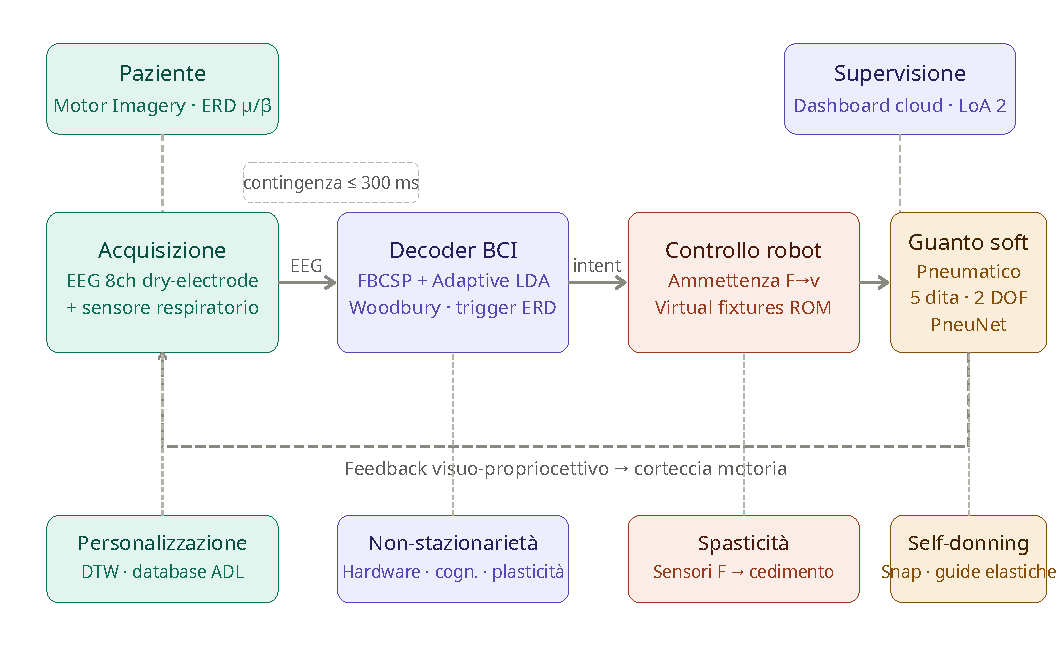
\includegraphics[width=\textwidth]{bci_glove_system_diagram_v2.pdf}
    \caption{Architettura closed-loop del sistema BCI-SRG. I quattro blocchi
    principali rappresentano: (1) il modulo di acquisizione EEG con sincronizzazione
    respiratoria; (2) il decoder BCI basato su FBCSP e LDA adattivo; (3) il modulo
    di controllo sicurezza con virtual fixtures e ammettenza; (4) il guanto soft
    pneumatico. La freccia tratteggiata chiude il loop riportando il feedback
    visuo-propriocettivo alla corteccia motoria. In alto: supervisione asincrona del
    terapista. La latenza complessiva target è $\leq 300$\,ms per garantire la
    contingenza Hebbiana \cite{biasiucci2018brain}.}
    \label{fig:architettura}
\end{figure}

\begin{figure}[ht]
    \centering
    % Inserire qui screenshot/render del modello URDF con joint limits annotati
    \caption{Modello cinematico URDF del guanto (dito singolo). I limiti articolari
    codificati (MCP $0$--$90°$, PIP $0$--$100°$, DIP $0$--$80°$) definiscono i
    parametri operativi delle virtual fixtures implementate nel firmware di controllo.}
    \label{fig:urdf}
\end{figure}

\end{document}% ---------------------------------------------------------------